\renewcommand{\theequation}{\theenumi}
\begin{enumerate}[label=\arabic*.,ref=\thesubsection.\theenumi]
\numberwithin{equation}{enumi}
%\chapter{The Optimum Receiver}
%\item Angles opposite to equal sides of a triangle are equal. 
%\label{prob:tri_ang_side_eq}
%\\
%\solution Using the sine formula in \eqref{eq:tri_sin_form},%
%\begin{align}
%\frac{\sin A}{a} = \frac{\sin B}{b}
%\end{align}
%%
%Thus, if $A=B$, $\sin A = \sin B \implies a =b$.
%\\
%\solution Use \eqref{eq:tri_sin_form} and the argument in Problem \ref{prob:tri_ang_side_eq}
%
\item  Each angle of an equilateral triangle is of 60$\degree$. 
\\
\solution 
\begin{enumerate}
\begin{figure}[!ht]
\centering
\resizebox{\columnwidth}{!}{\begin{tikzpicture}
[scale=2,>=stealth,point/.style={draw,circle,fill = black,inner sep=0.5pt},]

%Triangle sides
\def\a{4}
\def\b{4}
\def\c{4}
 
%Coordinates of A
\def\p{2}
\def\q{{sqrt(\c^2-\p^2)}}

%Labeling points
\node (A) at (\p,\q)[point,label=above right:$A$] {};
\node (B) at (0, 0)[point,label=below left:$B$] {};
\node (C) at (\a, 0)[point,label=below right:$C$] {};

%Drawing triangle ABC
\draw (A) -- node[left, xshift=-5mm,yshift=5mm] {$\textrm{a}$} (B) -- node[below, yshift=-5mm] {$\textrm{a}$} (C) -- node[above right,xshift=2mm,yshift=5mm] {$\textrm{a}$} (A);


%Angles
\tkzFillAngle[fill=green!60,size=.5](C,B,A)

%
\tkzFillAngle[fill=red!60,size=.5](A,C,B)

%%
\tkzFillAngle[fill=orange!60,size=.5](B,A,C)
%
%\tkzFillAngle[fill=blue!60,size=.3](E,A,F)
\end{tikzpicture}

}
\caption{}
\label{fig:8.1.1_similar}	
\end{figure}


\item {\em Construction: } See Fig. \ref{fig:8.1.1_similar}.
The input parameters are
\begin{multline}
 \vec{B}= \myvec{0\\0},
\vec{C}=\myvec{a\\0},
\vec{A}=a\myvec{\cos 60\degree\\ \sin 60\degree}
\end{multline}

\item {\em Proof: } Using the cosine formula,
%
\begin{align}
\cos \phase{ABC} &= \frac{a^2 +a^2 - a^2}{2a^2}
\\
&= \frac{1}{2}
\\
\implies  \phase{ABC} &= 60 \degree
\end{align}
%


\end{enumerate}
%%
%\begin{align}
%A=B=C.&
%\\
%\because A+B+C = 180\degree, 3A = 180\degree&
%\\
%\implies A = 60\degree&
%\end{align}
%


%\subsection{Problem}
\item Triangles on the same base (or equal bases) and between the same parallels are equal in area.
\begin{enumerate}
\begin{figure}[!ht]
\centering
\resizebox{\columnwidth}{!}{\renewcommand{\theequation}{\theenumi}
\begin{enumerate}[label=\thesubsection.\arabic*.,ref=\thesubsection.\theenumi]
\numberwithin{equation}{enumi}
	%
%
\item 
%
Draw a circle of radius 3 units.Take two points P and Q on one its extended diameter each at a distance of 7 units from its centre. Draw tangents to the circle from these two points P and Q. 
\\
\solution The given parameters are listed in Table \ref{tab:table1}
%
\begin{table}[!ht]
\begin{center}
\begin{tabular}{ | m{2cm} | m{2cm} |} 
\hline
 & Circle \\
\hline
Centre  & $\vec{O}$=\myvec{0\\0} \\ 
\hline
Radius & $r$=3  \\ 
\hline
Radius & $d$=7  \\ 
\hline
\end{tabular}
\end{center}
\caption{Input values}
\label{tab:table1}
\end{table}
%
\begin{lemma}
  \label{lemma/linman/circ/contact/final}
  The points of contact for the tangent drawn from a point 
%
\begin{align}
  \vec{P} = d\vec{e}_1, \text{ where } \vec{e}_1 = \myvec{1\\0}
  \end{align}
  %
  to the circle are given by 
  \begin{align}
    \vec{x} = \frac{r^2}{d}\vec{e}_1  \pm r\sqrt{1 - \frac{r^2}{d^2}} \vec{e}_2
    \label{linman/circ/contact/final}
   \end{align}
%   
\end{lemma}
If $\vec{x}$ be a point of contact for the tangent from $\vec{P}$, 
\begin{align}
PR &\perp RO
\\
 \implies (\vec{O}-\vec{x})^{\top} (\vec{x}-\vec{P}) &= 0
 \\
 \text{or, }  \vec{P}^{\top} \vec{x} &=\norm{\vec{x}}^2 = r^2
 \\
 \implies \vec{e}_1^{\top} \vec{x} &= \frac{r^2}{d}
  \end{align}
  $\because \vec{O} = 0$.  The above equation can be expressed in parametric form as 
 \begin{align}
  \vec{x} = \frac{r^2}{d}\vec{e}_1 + \lambda \vec{e}_2
  \label{linman/circ/contact}
 \end{align}
 Substituting the above in 
 \begin{align}
  \norm{\vec{x}}^2 = r^2,
 \end{align}
 yields
\begin{align}
\norm{\frac{r^2}{d}\vec{e}_1 + \lambda \vec{e}_2}^2&=r^2
\\
\implies \lambda^2 &= r^2\sbrak{1 - \frac{r^2}{d^2}}
\\
\text{or, }\lambda &= \pm r\sqrt{1 - \frac{r^2}{d^2}}
\end{align}
%
Substituting $\lambda $ in \eqref{linman/circ/contact} yields \eqref{linman/circ/contact/final}.  Fig.  \ref{fig:Tangent lines to circle of radius 3 units.} shows all possible tangents
and their points of contact after substituting the numerical values in \eqref{linman/circ/contact/final}.
%
\begin{figure}[ht]
  \centering
  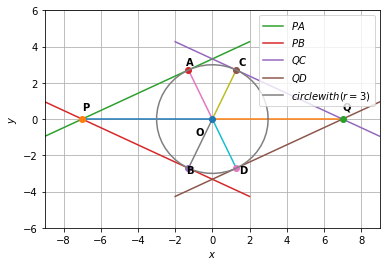
\includegraphics[width=\columnwidth]{solutions/su2021/circle/2/57/FIGURE3.png}
  \caption{Tangent lines to circle of radius 3 units.}
  \label{fig:Tangent lines to circle of radius 3 units.}
\end{figure}
%
\item Draw a  pair of tangents to a circle of radius 5 units  which are inclined to each other at an angle of $60\degree$.
\\
\solution  The angle between the tangents from $\vec{P}$ is given by 
\begin{lemma}
  Given a circle of radius $r$ and angle $\theta$ between the tangents, the intersection of the tangents and points of contact are
  given by Lemma   \ref{lemma/linman/circ/contact/final}  where 
  \begin{align}
    \implies d &= r\sin \frac{\theta}{2}
  \end{align}
%  
\end{lemma}
\begin{proof}
  From Fig.  \ref{fig:Tangent lines to circle of radius 3 units.},
\begin{align}
  \sin \frac{\theta}{2} &= \frac{r}{d}
  \\
  \implies d &= r\sin \frac{\theta}{2}
\end{align}
\end{proof}
Substituting numerical values and plotting, we obtain Fig. \ref{fig:Tangent lines to circle of radius 5 units.}.
%
\begin{figure}[ht]
  \centering
  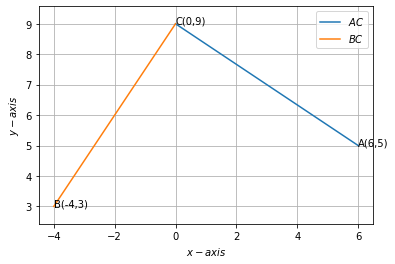
\includegraphics[width=\columnwidth]{solutions/su2021/circle/2/58/download.png}
  \caption{Tangent lines to circle of radius 5 units.}
  \label{fig:Tangent lines to circle of radius 5 units.}
\end{figure}   

\end{enumerate}
}
\caption{}
\label{fig:8.5.49_circle}	
\end{figure}
%
\item {\em Construction: }See Fig. \ref{fig:8.5.49_circle}.  The input parameters are
%
\begin{align}
\label{eq:8.5.49_constr_o}
\vec{O} &= \myvec{0\\0} 
\\
\vec{C} &= \myvec{r\\0} 
\label{eq:8.5.49_constr_c}
\end{align}
Then, 
%
\begin{align}
\label{eq:8.5.49_constr_a}
\vec{A} &= r\myvec{\cos \beta \\ -\sin \beta} 
\end{align}

\subitem Equal chords subtend equal angles at the centre.  Hence 
\begin{align}
\phase{EOC} &= \phase{AOD} = \frac{360 \degree - \alpha -\beta}{2}
\\
&= 180\degree - \frac{\alpha+\beta}{2}
\end{align}
Thus, 
\begin{align}
\vec{D} &= r\myvec{\cos \brak{180^{\circ}-\frac{\alpha+\beta}{2}+\alpha} \\ \sin \brak{180^{\circ}-\frac{\alpha+\beta}{2}+\alpha}} 
\\
 &= r\myvec{-\cos \frac{\alpha-\beta}{2} \\ -\sin \frac{\alpha-\beta}{2}}
\label{eq:8.5.49_constr_d}
\\
\vec{E} &= r\myvec{\cos \brak{180^{\circ}-\frac{\alpha+\beta}{2}} \\ \sin \brak{180^{\circ}-\frac{\alpha+\beta}{2}}}
\\
 &= r\myvec{-\cos \frac{\alpha+\beta}{2} \\ \sin \frac{\alpha+\beta}{2}}
\label{eq:8.5.49_constr_e}
\end{align}
\subitem $\vec{B}$ can be found as the intersection of $AD$ and $CE$.

The given curve 
\begin{align}
	y =\frac{1}{x-1}
\end{align}
can be expressed as 
\begin{align}
	xy - y - 1 = 0 \label{eq:solutions/1/14/eq:hyperbola}
\end{align}
Hence, we have
\begin{align}
	\vec{V} = \frac{1}{2}\myvec{0 & 1 \\ 1 & 0}, 
	\vec{u} = \frac{1}{2}\myvec{0 \\-1},
	f = -1
\end{align}
Since $\mydet{\vec{V}} < 0$, the equation \eqref{eq:solutions/1/14/eq:hyperbola} represents hyperbola.
To find the values of $\lambda_1$ and $\lambda_2$, consider the characteristic equation,
\begin{align}
	\mydet{\lambda\vec{I} - \vec{V}} &= 0\\
	\implies \mydet{\myvec{\lambda & 0\\0 & \lambda} - \myvec{0 & \frac{1}{2} \\ \frac{1}{2} & 0}} &= 0\\
	\implies \mydet{ \lambda & \frac{-1}{2} \\ \frac{-1}{2} & \lambda} &= 0\\
	\implies \lambda_1 &= \frac{1}{2} , \lambda_2 = \frac{-1}{2}
\end{align}
In addition, given the slope -1, the direction and normal vectors are given by 
\begin{align}
	\vec{m} = \myvec{1 \\ -1} \\
	\vec{n} = \myvec{ 1 \\ 1}
\end{align}
The parameters of hyperbola are as follows:
\begin{align}
	\vec{c} &= -\vec{V}^{-1}\vec{u} \\
	&= -\myvec{0 & 2\\ 2 & 0}\myvec{0 \\ -\frac{1}{2}} \\
	&= \myvec{1 \\ 0}\\
	axes &= \begin{cases}
	\sqrt{\frac{\vec{u}^T\vec{V}^{-1}\vec{u} - f}{\lambda_1}} = \sqrt{2}\\
 \sqrt{\frac{f-\vec{u}^T\vec{V}^{-1}\vec{u}}{\lambda_2}} = \sqrt{2}
\end{cases}
\end{align}
which represents the standard hyperbola equation,
\begin{align}
	\frac{x^2}{2} - \frac{x^2}{2} = 1
\end{align}
The points of contact are given by 
\begin{align}
  \tiny{K} &=\pm \sqrt{\frac{\vec{u}^T\vec{V}^{-1}\vec{u} - f}{\vec{n}^T\vec{V}^{-1}\vec{n}}}
  = \pm \frac{1}{2}\\
  \vec{q} &= \vec{V}^{-1}(k\vec{n}-\vec{u})\\
  \vec{q_1} &= \myvec{0 & 2\\2 & 0} \sbrak{\frac{1}{2}\myvec{1 \\ 1} - \myvec{0\\ \frac{-1}{2}}}\\
  &= \myvec{2 \\ 1}\\
  \vec{q_2} &= \myvec{0 & 2\\2 & 0} \sbrak{\frac{-1}{2}\myvec{1 \\ 1} - \myvec{0\\ \frac{-1}{2}}}\\
  &= \myvec{0 \\ -1}
\end{align} 
$\therefore$ The tangents are given by
\begin{align}
	\myvec{1 & 1} \brak{\vec{x} - \myvec{2 \\ 1}} = 0 \\
	\myvec{1 & 1} \brak{\vec{x} - \myvec{0 \\ -1}} = 0
\end{align}
The desired equations of all lines having slope -1 that are tangents to the curve $\frac{1}{x-1}, x \neq 1$ are given by
\begin{align}
	\myvec{1 & 1}\vec{x} &= 3 \\
	\myvec{1 & 1}\vec{x} &= -1 
\end{align}
The above results are verified in the following figure.
\begin{figure}[h!] \label{eq:solutions/1/14/fig:tangents}
	\centering
	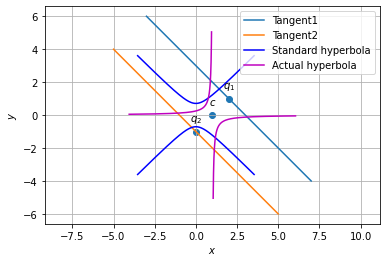
\includegraphics[width=\columnwidth]{./solutions/1/14/graph7.png}
	\caption{The standard and actual hyperbola.}
\end{figure}

\end{enumerate}
\item Triangles on the same base (or equal bases) and having equal areas lie between the same parallels.
\item In $\triangle ABC, D, E$ and $F$ are respectively the mid-points of sides $AB, BC$ and $CA $. Show that $\triangle ABC$ is divided into four congruent triangles by joining $D, E$ and $F$.
\item  The line-segment joining the mid-points of any two sides of a triangle is parallel to the third side and is half of it.
\label{prob:tri_mid_similar}
%\label{prob:quad_similar}
%%
%\\
%\solution If $DE$ is the lie joining he mid points of $\triangle ABC$,  use cosine formula to find the lengths of $DE$ and $BC$. Then use cosine formula to show that all angles of $\triangle ADE$ are equal to the corresponding angles of $\triangle ABC$.
%
\item  A line through the mid-point of a side of a triangle parallel to another side 
bisects the third side.
%\\
%\solution Use cosine formula.

\item ABC is a triangle right angled at $C$. A line through the mid-point $M$ of hypotenuse $AB$ and parallel to $BC$ intersects $AC$ at $D$. Show that (i) $D$ is the mid-point of $AC$
(ii) $MD \perp AC$ (iii) $CM = MA = \frac{1}{2}AB$

\item  Sides opposite to equal angles of a triangle are equal. 
%\\
%\solution Use \eqref{eq:tri_sin_form} and the argument in Problem \ref{prob:tri_ang_side_eq}
%
\item  Each angle of an equilateral triangle is of 60$\degree$. 
%\\
%\solution In an equilateral $\triangle$, 
%%
%\begin{align}
%A=B=C.&
%\\
%\because A+B+C = 180\degree, 3A = 180\degree&
%\\
%\implies A = 60\degree&
%\end{align}
%
\item Using cosine formula in an equilateral $\triangle$, show that $\cos 60\degree = \frac{1}{2} $.  
\item Using \eqref{eq:tri_sin_cos_id}, show that $\sin 60\degree = \frac{\sqrt{3}}{2} $.
\item Find  $\sin 30\degree$ and  $\sin 30\degree$ using \eqref{eq:tri_90-ang}.
%\subsection{Problem}
\item Triangles on the same base (or equal bases) and between the same parallels are equal in area.
\item Triangles on the same base (or equal bases) and having equal areas lie between the same parallels.
\item In $\triangle ABC$, the bisector $AD$ of $\angle  A$ is perpendicular to side $BC$. Show that $AB = AC$ and $\triangle ABC$ is isosceles.
\item $E$ and $F$ are respectively the mid-points of equal sides $AB$ and AC of $\triangle ABC$. Show that $BF = CE$. 
\item In an isosceles $\triangle ABC$ with $AB$ = AC, D and E are points on $BC$ such that $BE = CD$. Show that $AD = AE$. 
%
\item $AB$ is a line-segment. $P$ and $Q$ are points on opposite sides of $AB$ such that each of them is equidistant from the points $A$ and $B$. Show that the line $PQ $ is the perpendicular bisector of $AB$.
%
\item $P$ is a point equidistant from two lines $l$ and $m$ intersecting at point $A$.  Show that the line  $AP$  bisects the angle between them.
%
\item $D$ is a point on side $BC$ of $\triangle  ABC$ such that $AD = AC$. Show that $AB > AD$

%
\item $AB$ is a line segment and line $l$ is its perpendicular bisector. If a point $P$ lies on $l$, show that $P$ is equidistant from $A$ and $B$.
\item Line-segment $AB$ is parallel to another line-segment $CD$. $O$ is the mid-point of $AD$. Show that 
\begin{enumerate}
\item  $\triangle AOB \cong \triangle DOC$ 
\item  $O$ is also the mid-point of $BC$.
\end{enumerate}
%
\item In quadrilateral $ACBD, AC = AD$ and $AB$ bisects $\angle  A$. Show that $\triangle  ABC \cong \triangle  ABD$. What can you say about $BC$ and $BD$?
\label{prob:8.1.23}
\begin{enumerate}
\begin{figure}[!ht]
\centering
\resizebox{\columnwidth}{!}{\renewcommand{\theequation}{\theenumi}
\begin{enumerate}[label=\thesubsection.\arabic*.,ref=\thesubsection.\theenumi]
\numberwithin{equation}{enumi}
	%
%
\item 
%
Draw a circle of radius 3 units.Take two points P and Q on one its extended diameter each at a distance of 7 units from its centre. Draw tangents to the circle from these two points P and Q. 
\\
\solution The given parameters are listed in Table \ref{tab:table1}
%
\begin{table}[!ht]
\begin{center}
\begin{tabular}{ | m{2cm} | m{2cm} |} 
\hline
 & Circle \\
\hline
Centre  & $\vec{O}$=\myvec{0\\0} \\ 
\hline
Radius & $r$=3  \\ 
\hline
Radius & $d$=7  \\ 
\hline
\end{tabular}
\end{center}
\caption{Input values}
\label{tab:table1}
\end{table}
%
\begin{lemma}
  \label{lemma/linman/circ/contact/final}
  The points of contact for the tangent drawn from a point 
%
\begin{align}
  \vec{P} = d\vec{e}_1, \text{ where } \vec{e}_1 = \myvec{1\\0}
  \end{align}
  %
  to the circle are given by 
  \begin{align}
    \vec{x} = \frac{r^2}{d}\vec{e}_1  \pm r\sqrt{1 - \frac{r^2}{d^2}} \vec{e}_2
    \label{linman/circ/contact/final}
   \end{align}
%   
\end{lemma}
If $\vec{x}$ be a point of contact for the tangent from $\vec{P}$, 
\begin{align}
PR &\perp RO
\\
 \implies (\vec{O}-\vec{x})^{\top} (\vec{x}-\vec{P}) &= 0
 \\
 \text{or, }  \vec{P}^{\top} \vec{x} &=\norm{\vec{x}}^2 = r^2
 \\
 \implies \vec{e}_1^{\top} \vec{x} &= \frac{r^2}{d}
  \end{align}
  $\because \vec{O} = 0$.  The above equation can be expressed in parametric form as 
 \begin{align}
  \vec{x} = \frac{r^2}{d}\vec{e}_1 + \lambda \vec{e}_2
  \label{linman/circ/contact}
 \end{align}
 Substituting the above in 
 \begin{align}
  \norm{\vec{x}}^2 = r^2,
 \end{align}
 yields
\begin{align}
\norm{\frac{r^2}{d}\vec{e}_1 + \lambda \vec{e}_2}^2&=r^2
\\
\implies \lambda^2 &= r^2\sbrak{1 - \frac{r^2}{d^2}}
\\
\text{or, }\lambda &= \pm r\sqrt{1 - \frac{r^2}{d^2}}
\end{align}
%
Substituting $\lambda $ in \eqref{linman/circ/contact} yields \eqref{linman/circ/contact/final}.  Fig.  \ref{fig:Tangent lines to circle of radius 3 units.} shows all possible tangents
and their points of contact after substituting the numerical values in \eqref{linman/circ/contact/final}.
%
\begin{figure}[ht]
  \centering
  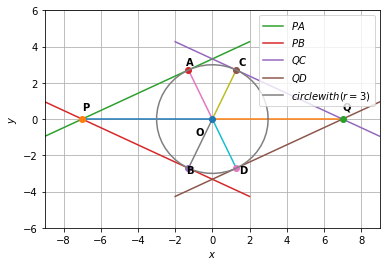
\includegraphics[width=\columnwidth]{solutions/su2021/circle/2/57/FIGURE3.png}
  \caption{Tangent lines to circle of radius 3 units.}
  \label{fig:Tangent lines to circle of radius 3 units.}
\end{figure}
%
\item Draw a  pair of tangents to a circle of radius 5 units  which are inclined to each other at an angle of $60\degree$.
\\
\solution  The angle between the tangents from $\vec{P}$ is given by 
\begin{lemma}
  Given a circle of radius $r$ and angle $\theta$ between the tangents, the intersection of the tangents and points of contact are
  given by Lemma   \ref{lemma/linman/circ/contact/final}  where 
  \begin{align}
    \implies d &= r\sin \frac{\theta}{2}
  \end{align}
%  
\end{lemma}
\begin{proof}
  From Fig.  \ref{fig:Tangent lines to circle of radius 3 units.},
\begin{align}
  \sin \frac{\theta}{2} &= \frac{r}{d}
  \\
  \implies d &= r\sin \frac{\theta}{2}
\end{align}
\end{proof}
Substituting numerical values and plotting, we obtain Fig. \ref{fig:Tangent lines to circle of radius 5 units.}.
%
\begin{figure}[ht]
  \centering
  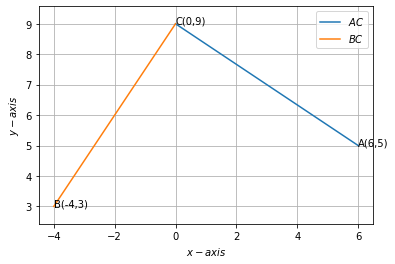
\includegraphics[width=\columnwidth]{solutions/su2021/circle/2/58/download.png}
  \caption{Tangent lines to circle of radius 5 units.}
  \label{fig:Tangent lines to circle of radius 5 units.}
\end{figure}   

\end{enumerate}
}
\caption{}
\label{fig:8.5.49_circle}	
\end{figure}
%
\item {\em Construction: }See Fig. \ref{fig:8.5.49_circle}.  The input parameters are
%
\begin{align}
\label{eq:8.5.49_constr_o}
\vec{O} &= \myvec{0\\0} 
\\
\vec{C} &= \myvec{r\\0} 
\label{eq:8.5.49_constr_c}
\end{align}
Then, 
%
\begin{align}
\label{eq:8.5.49_constr_a}
\vec{A} &= r\myvec{\cos \beta \\ -\sin \beta} 
\end{align}

\subitem Equal chords subtend equal angles at the centre.  Hence 
\begin{align}
\phase{EOC} &= \phase{AOD} = \frac{360 \degree - \alpha -\beta}{2}
\\
&= 180\degree - \frac{\alpha+\beta}{2}
\end{align}
Thus, 
\begin{align}
\vec{D} &= r\myvec{\cos \brak{180^{\circ}-\frac{\alpha+\beta}{2}+\alpha} \\ \sin \brak{180^{\circ}-\frac{\alpha+\beta}{2}+\alpha}} 
\\
 &= r\myvec{-\cos \frac{\alpha-\beta}{2} \\ -\sin \frac{\alpha-\beta}{2}}
\label{eq:8.5.49_constr_d}
\\
\vec{E} &= r\myvec{\cos \brak{180^{\circ}-\frac{\alpha+\beta}{2}} \\ \sin \brak{180^{\circ}-\frac{\alpha+\beta}{2}}}
\\
 &= r\myvec{-\cos \frac{\alpha+\beta}{2} \\ \sin \frac{\alpha+\beta}{2}}
\label{eq:8.5.49_constr_e}
\end{align}
\subitem $\vec{B}$ can be found as the intersection of $AD$ and $CE$.

The given curve 
\begin{align}
	y =\frac{1}{x-1}
\end{align}
can be expressed as 
\begin{align}
	xy - y - 1 = 0 \label{eq:solutions/1/14/eq:hyperbola}
\end{align}
Hence, we have
\begin{align}
	\vec{V} = \frac{1}{2}\myvec{0 & 1 \\ 1 & 0}, 
	\vec{u} = \frac{1}{2}\myvec{0 \\-1},
	f = -1
\end{align}
Since $\mydet{\vec{V}} < 0$, the equation \eqref{eq:solutions/1/14/eq:hyperbola} represents hyperbola.
To find the values of $\lambda_1$ and $\lambda_2$, consider the characteristic equation,
\begin{align}
	\mydet{\lambda\vec{I} - \vec{V}} &= 0\\
	\implies \mydet{\myvec{\lambda & 0\\0 & \lambda} - \myvec{0 & \frac{1}{2} \\ \frac{1}{2} & 0}} &= 0\\
	\implies \mydet{ \lambda & \frac{-1}{2} \\ \frac{-1}{2} & \lambda} &= 0\\
	\implies \lambda_1 &= \frac{1}{2} , \lambda_2 = \frac{-1}{2}
\end{align}
In addition, given the slope -1, the direction and normal vectors are given by 
\begin{align}
	\vec{m} = \myvec{1 \\ -1} \\
	\vec{n} = \myvec{ 1 \\ 1}
\end{align}
The parameters of hyperbola are as follows:
\begin{align}
	\vec{c} &= -\vec{V}^{-1}\vec{u} \\
	&= -\myvec{0 & 2\\ 2 & 0}\myvec{0 \\ -\frac{1}{2}} \\
	&= \myvec{1 \\ 0}\\
	axes &= \begin{cases}
	\sqrt{\frac{\vec{u}^T\vec{V}^{-1}\vec{u} - f}{\lambda_1}} = \sqrt{2}\\
 \sqrt{\frac{f-\vec{u}^T\vec{V}^{-1}\vec{u}}{\lambda_2}} = \sqrt{2}
\end{cases}
\end{align}
which represents the standard hyperbola equation,
\begin{align}
	\frac{x^2}{2} - \frac{x^2}{2} = 1
\end{align}
The points of contact are given by 
\begin{align}
  \tiny{K} &=\pm \sqrt{\frac{\vec{u}^T\vec{V}^{-1}\vec{u} - f}{\vec{n}^T\vec{V}^{-1}\vec{n}}}
  = \pm \frac{1}{2}\\
  \vec{q} &= \vec{V}^{-1}(k\vec{n}-\vec{u})\\
  \vec{q_1} &= \myvec{0 & 2\\2 & 0} \sbrak{\frac{1}{2}\myvec{1 \\ 1} - \myvec{0\\ \frac{-1}{2}}}\\
  &= \myvec{2 \\ 1}\\
  \vec{q_2} &= \myvec{0 & 2\\2 & 0} \sbrak{\frac{-1}{2}\myvec{1 \\ 1} - \myvec{0\\ \frac{-1}{2}}}\\
  &= \myvec{0 \\ -1}
\end{align} 
$\therefore$ The tangents are given by
\begin{align}
	\myvec{1 & 1} \brak{\vec{x} - \myvec{2 \\ 1}} = 0 \\
	\myvec{1 & 1} \brak{\vec{x} - \myvec{0 \\ -1}} = 0
\end{align}
The desired equations of all lines having slope -1 that are tangents to the curve $\frac{1}{x-1}, x \neq 1$ are given by
\begin{align}
	\myvec{1 & 1}\vec{x} &= 3 \\
	\myvec{1 & 1}\vec{x} &= -1 
\end{align}
The above results are verified in the following figure.
\begin{figure}[h!] \label{eq:solutions/1/14/fig:tangents}
	\centering
	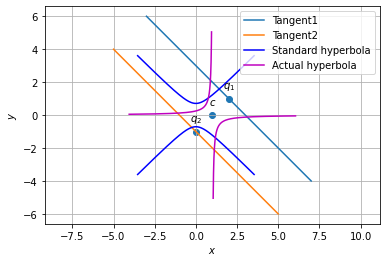
\includegraphics[width=\columnwidth]{./solutions/1/14/graph7.png}
	\caption{The standard and actual hyperbola.}
\end{figure}

\end{enumerate}

%
\item $ABCD$ is a quadrilateral in which $AD = BC$ and $\angle  DAB = \angle  CBA$ . Prove that
\begin{enumerate}
\item  $\triangle  ABD \cong  \triangle  BAC $
\item $ BD = AC $
\item  $\angle  ABD = \angle  BAC$.
\end{enumerate}
%
\item $l$ and $m$ are two parallel lines intersected by another pair of parallel lines p and q 
to form the quadrilateral $ABCD$. Show that $\triangle  ABC \cong  \triangle  CDA$.
%
\item Line $l$ is the bisector of $ \angle  A$ and $B$ is any point on $l$. $BP$ and $BQ$ are perpendiculars from $B$ to the arms of $\angle  A$. Show that: 
\begin{enumerate}
\item  $\triangle  APB \cong  \triangle  AQB$ 
\item  $BP = BQ$ or $B$ is equidistant from the arms of $\angle  A$.
\end{enumerate}
%
\begin{enumerate}
\begin{figure}[!ht]
\centering
\resizebox{\columnwidth}{!}{%Exercise 8.1 prob 47
\begin{tikzpicture}
[scale=0.5,>=stealth,point/.style={draw,circle,fill = black,inner sep=0.5pt},]
%\tikzset{shift={(-3,0)}}
%Triangle sides
\def\a{4}
\def\c{9}
\def\xA{4}
\def\h{3}
\def\k{1}
%\def\c{7.5}
\def\yE{\h/2}
%Labeling points
\node (D) at (0,0)[point,label=below left:$D$] {};
\node (B) at ({\xA+\a}, \h )[point,label=above right:$B$] {};
\node (C) at (\c, 0)[point,label=below right:$C$] {};
%\node (E) at (2, \yE)
%\node (F) at (8.5, \yE)[point,label=below right:$F$] {};
%\node (M) at (\xA,\yE)[point,label=above right:$M$] {};
%\node (N) at ({\xA+\a}, \yE)[point,label=above left:$N$] {};
%\node (X) at (\xA , 0)[point,label=below left:$X$] {};
%\node (Y) at ({\xA+\a}, 0)[point,label=below right:$Y$] {};
\node (A) at (\xA , \h)[point,label=above left:$A$] {};
\node (E) at ($(D)!0.5!(A)$)[point,label=above left:$E$] {};
\node (F) at ($(B)!0.5!(C)$)[point,label=above right:$F$] {};



%A



%Drawing parallelogram ABCD
\draw (A) -- (B)--(C) --(D)--(A);
%\draw (A) --(X);
\draw (E) --(F);
\draw(A)--node[right]{$\textrm{k}$} (E)--node[right]{$\textrm{1}$} (D);
\draw(B)--node[left]{$\textrm{m}$} (F)--node[left]{$\textrm{1}$} (C);


%\draw (B) --(Y);
%marking right angles
%\tkzMarkRightAngle[fill=green!20,size=.2](D,X,A)
%\tkzMarkRightAngle[fill=green!20,size=.2](C,Y,B)


%
\end{tikzpicture}
}
\caption{}
\label{fig:8.1.47_trapezium_ABCD}	
\end{figure}

\item {\em Construction: }See Fig. \ref{fig:8.1.47_trapezium_ABCD}.
The input parameters are
\begin{align}
\label{eq:8.1.47_constr_d}
\vec{D} &= \myvec{0\\0} 
\\
\vec{C} &= \myvec{c\\0} 
\\
\vec{A} &= \myvec{p\\q} 
\\
\vec{B} &= \myvec{b\\q}, \quad b < c 
\label{eq:8.1.47_constr_c}
\end{align}
%
For $0 < k < 1$, 
\begin{align}
\label{eq:8.1.47_constr_e}
\vec{E} &= \frac{{k\vec{D} +\vec{A}}}{k+1}
\\
\vec{F} &= \frac{{k\vec{C} +\vec{B}}}{k+1}
\label{eq:8.1.47_constr_f}
\end{align}


The given curve 
\begin{align}
	y =\frac{1}{x-1}
\end{align}
can be expressed as 
\begin{align}
	xy - y - 1 = 0 \label{eq:solutions/1/14/eq:hyperbola}
\end{align}
Hence, we have
\begin{align}
	\vec{V} = \frac{1}{2}\myvec{0 & 1 \\ 1 & 0}, 
	\vec{u} = \frac{1}{2}\myvec{0 \\-1},
	f = -1
\end{align}
Since $\mydet{\vec{V}} < 0$, the equation \eqref{eq:solutions/1/14/eq:hyperbola} represents hyperbola.
To find the values of $\lambda_1$ and $\lambda_2$, consider the characteristic equation,
\begin{align}
	\mydet{\lambda\vec{I} - \vec{V}} &= 0\\
	\implies \mydet{\myvec{\lambda & 0\\0 & \lambda} - \myvec{0 & \frac{1}{2} \\ \frac{1}{2} & 0}} &= 0\\
	\implies \mydet{ \lambda & \frac{-1}{2} \\ \frac{-1}{2} & \lambda} &= 0\\
	\implies \lambda_1 &= \frac{1}{2} , \lambda_2 = \frac{-1}{2}
\end{align}
In addition, given the slope -1, the direction and normal vectors are given by 
\begin{align}
	\vec{m} = \myvec{1 \\ -1} \\
	\vec{n} = \myvec{ 1 \\ 1}
\end{align}
The parameters of hyperbola are as follows:
\begin{align}
	\vec{c} &= -\vec{V}^{-1}\vec{u} \\
	&= -\myvec{0 & 2\\ 2 & 0}\myvec{0 \\ -\frac{1}{2}} \\
	&= \myvec{1 \\ 0}\\
	axes &= \begin{cases}
	\sqrt{\frac{\vec{u}^T\vec{V}^{-1}\vec{u} - f}{\lambda_1}} = \sqrt{2}\\
 \sqrt{\frac{f-\vec{u}^T\vec{V}^{-1}\vec{u}}{\lambda_2}} = \sqrt{2}
\end{cases}
\end{align}
which represents the standard hyperbola equation,
\begin{align}
	\frac{x^2}{2} - \frac{x^2}{2} = 1
\end{align}
The points of contact are given by 
\begin{align}
  \tiny{K} &=\pm \sqrt{\frac{\vec{u}^T\vec{V}^{-1}\vec{u} - f}{\vec{n}^T\vec{V}^{-1}\vec{n}}}
  = \pm \frac{1}{2}\\
  \vec{q} &= \vec{V}^{-1}(k\vec{n}-\vec{u})\\
  \vec{q_1} &= \myvec{0 & 2\\2 & 0} \sbrak{\frac{1}{2}\myvec{1 \\ 1} - \myvec{0\\ \frac{-1}{2}}}\\
  &= \myvec{2 \\ 1}\\
  \vec{q_2} &= \myvec{0 & 2\\2 & 0} \sbrak{\frac{-1}{2}\myvec{1 \\ 1} - \myvec{0\\ \frac{-1}{2}}}\\
  &= \myvec{0 \\ -1}
\end{align} 
$\therefore$ The tangents are given by
\begin{align}
	\myvec{1 & 1} \brak{\vec{x} - \myvec{2 \\ 1}} = 0 \\
	\myvec{1 & 1} \brak{\vec{x} - \myvec{0 \\ -1}} = 0
\end{align}
The desired equations of all lines having slope -1 that are tangents to the curve $\frac{1}{x-1}, x \neq 1$ are given by
\begin{align}
	\myvec{1 & 1}\vec{x} &= 3 \\
	\myvec{1 & 1}\vec{x} &= -1 
\end{align}
The above results are verified in the following figure.
\begin{figure}[h!] \label{eq:solutions/1/14/fig:tangents}
	\centering
	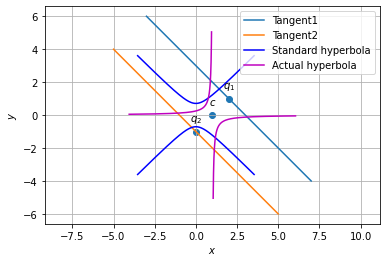
\includegraphics[width=\columnwidth]{./solutions/1/14/graph7.png}
	\caption{The standard and actual hyperbola.}
\end{figure}

\end{enumerate}

\item $ABCE$ is a quadrilateral and $D$ is a point on $BC$ such that, $AC = AE, AB = AD$ and $\angle  BAD = \angle  EAC$. Show that $BC = DE$.
%
\item In right triangle $ABC$, right angled at $C, M$ is the mid-point of hypotenuse $AB$. $C$ is joined to $M$ and produced to a point $D$ such that $DM = CM$. Point $D$ is joined to point $B$.
Show that: 
\begin{enumerate}
\item $ \triangle  AMC \cong  \triangle  BMD $
\item $\angle  DBC$ is a right angle. 
\item $\triangle  DBC \cong  \triangle  ACB$
\item $ CM = \frac{1}{ 2} AB$
\end{enumerate}
%
See  Fig. \ref{fig:8.1.28}.
%\solution 
\begin{enumerate}
\begin{figure}[!ht]
\centering
\resizebox{\columnwidth}{!}{%Exercise 8.1 prob 47
\begin{tikzpicture}
[scale=0.5,>=stealth,point/.style={draw,circle,fill = black,inner sep=0.5pt},]
%\tikzset{shift={(-3,0)}}
%Triangle sides
\def\a{4}
\def\c{9}
\def\xA{4}
\def\h{3}
\def\k{1}
%\def\c{7.5}
\def\yE{\h/2}
%Labeling points
\node (D) at (0,0)[point,label=below left:$D$] {};
\node (B) at ({\xA+\a}, \h )[point,label=above right:$B$] {};
\node (C) at (\c, 0)[point,label=below right:$C$] {};
%\node (E) at (2, \yE)
%\node (F) at (8.5, \yE)[point,label=below right:$F$] {};
%\node (M) at (\xA,\yE)[point,label=above right:$M$] {};
%\node (N) at ({\xA+\a}, \yE)[point,label=above left:$N$] {};
%\node (X) at (\xA , 0)[point,label=below left:$X$] {};
%\node (Y) at ({\xA+\a}, 0)[point,label=below right:$Y$] {};
\node (A) at (\xA , \h)[point,label=above left:$A$] {};
\node (E) at ($(D)!0.5!(A)$)[point,label=above left:$E$] {};
\node (F) at ($(B)!0.5!(C)$)[point,label=above right:$F$] {};



%A



%Drawing parallelogram ABCD
\draw (A) -- (B)--(C) --(D)--(A);
%\draw (A) --(X);
\draw (E) --(F);
\draw(A)--node[right]{$\textrm{k}$} (E)--node[right]{$\textrm{1}$} (D);
\draw(B)--node[left]{$\textrm{m}$} (F)--node[left]{$\textrm{1}$} (C);


%\draw (B) --(Y);
%marking right angles
%\tkzMarkRightAngle[fill=green!20,size=.2](D,X,A)
%\tkzMarkRightAngle[fill=green!20,size=.2](C,Y,B)


%
\end{tikzpicture}
}
\caption{}
\label{fig:8.1.47_trapezium_ABCD}	
\end{figure}

\item {\em Construction: }See Fig. \ref{fig:8.1.47_trapezium_ABCD}.
The input parameters are
\begin{align}
\label{eq:8.1.47_constr_d}
\vec{D} &= \myvec{0\\0} 
\\
\vec{C} &= \myvec{c\\0} 
\\
\vec{A} &= \myvec{p\\q} 
\\
\vec{B} &= \myvec{b\\q}, \quad b < c 
\label{eq:8.1.47_constr_c}
\end{align}
%
For $0 < k < 1$, 
\begin{align}
\label{eq:8.1.47_constr_e}
\vec{E} &= \frac{{k\vec{D} +\vec{A}}}{k+1}
\\
\vec{F} &= \frac{{k\vec{C} +\vec{B}}}{k+1}
\label{eq:8.1.47_constr_f}
\end{align}


The given curve 
\begin{align}
	y =\frac{1}{x-1}
\end{align}
can be expressed as 
\begin{align}
	xy - y - 1 = 0 \label{eq:solutions/1/14/eq:hyperbola}
\end{align}
Hence, we have
\begin{align}
	\vec{V} = \frac{1}{2}\myvec{0 & 1 \\ 1 & 0}, 
	\vec{u} = \frac{1}{2}\myvec{0 \\-1},
	f = -1
\end{align}
Since $\mydet{\vec{V}} < 0$, the equation \eqref{eq:solutions/1/14/eq:hyperbola} represents hyperbola.
To find the values of $\lambda_1$ and $\lambda_2$, consider the characteristic equation,
\begin{align}
	\mydet{\lambda\vec{I} - \vec{V}} &= 0\\
	\implies \mydet{\myvec{\lambda & 0\\0 & \lambda} - \myvec{0 & \frac{1}{2} \\ \frac{1}{2} & 0}} &= 0\\
	\implies \mydet{ \lambda & \frac{-1}{2} \\ \frac{-1}{2} & \lambda} &= 0\\
	\implies \lambda_1 &= \frac{1}{2} , \lambda_2 = \frac{-1}{2}
\end{align}
In addition, given the slope -1, the direction and normal vectors are given by 
\begin{align}
	\vec{m} = \myvec{1 \\ -1} \\
	\vec{n} = \myvec{ 1 \\ 1}
\end{align}
The parameters of hyperbola are as follows:
\begin{align}
	\vec{c} &= -\vec{V}^{-1}\vec{u} \\
	&= -\myvec{0 & 2\\ 2 & 0}\myvec{0 \\ -\frac{1}{2}} \\
	&= \myvec{1 \\ 0}\\
	axes &= \begin{cases}
	\sqrt{\frac{\vec{u}^T\vec{V}^{-1}\vec{u} - f}{\lambda_1}} = \sqrt{2}\\
 \sqrt{\frac{f-\vec{u}^T\vec{V}^{-1}\vec{u}}{\lambda_2}} = \sqrt{2}
\end{cases}
\end{align}
which represents the standard hyperbola equation,
\begin{align}
	\frac{x^2}{2} - \frac{x^2}{2} = 1
\end{align}
The points of contact are given by 
\begin{align}
  \tiny{K} &=\pm \sqrt{\frac{\vec{u}^T\vec{V}^{-1}\vec{u} - f}{\vec{n}^T\vec{V}^{-1}\vec{n}}}
  = \pm \frac{1}{2}\\
  \vec{q} &= \vec{V}^{-1}(k\vec{n}-\vec{u})\\
  \vec{q_1} &= \myvec{0 & 2\\2 & 0} \sbrak{\frac{1}{2}\myvec{1 \\ 1} - \myvec{0\\ \frac{-1}{2}}}\\
  &= \myvec{2 \\ 1}\\
  \vec{q_2} &= \myvec{0 & 2\\2 & 0} \sbrak{\frac{-1}{2}\myvec{1 \\ 1} - \myvec{0\\ \frac{-1}{2}}}\\
  &= \myvec{0 \\ -1}
\end{align} 
$\therefore$ The tangents are given by
\begin{align}
	\myvec{1 & 1} \brak{\vec{x} - \myvec{2 \\ 1}} = 0 \\
	\myvec{1 & 1} \brak{\vec{x} - \myvec{0 \\ -1}} = 0
\end{align}
The desired equations of all lines having slope -1 that are tangents to the curve $\frac{1}{x-1}, x \neq 1$ are given by
\begin{align}
	\myvec{1 & 1}\vec{x} &= 3 \\
	\myvec{1 & 1}\vec{x} &= -1 
\end{align}
The above results are verified in the following figure.
\begin{figure}[h!] \label{eq:solutions/1/14/fig:tangents}
	\centering
	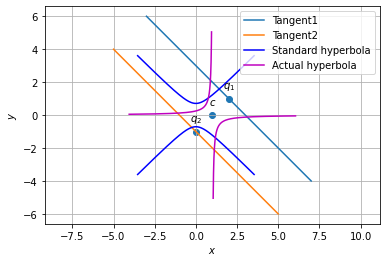
\includegraphics[width=\columnwidth]{./solutions/1/14/graph7.png}
	\caption{The standard and actual hyperbola.}
\end{figure}

\end{enumerate}

\item In an isosceles $\triangle ABC$, with $AB = AC$, the bisectors of $\angle B$ and $\angle C$ intersect each other at $O$. Join $A$ to $O$. Show that :
\begin{enumerate} 
\item $OB = OC$ 
\item $AO$ bisects $\angle A$
\end{enumerate}
\item In $\triangle ABC$, $AD$ is the perpendicular bisector of $BC$. Show that $\triangle ABC$ is an isosceles triangle in which $AB = AC$.
\item $ABC$ is an isosceles triangle in which altitudes $BE$ and $CF$ are drawn to equal sides $AC$ and $AB$ respectively . Show that these altitudes are equal.
%
\item $ABC$ is a triangle in which altitudes $BE$ and $CF$ to sides $AC$ and $AB$ are equal. Show that
%
\begin{enumerate} 
\item $\triangle  ABE \cong  \triangle  ACF $
\item  $AB = AC$, i.e., $ABC$ is an isosceles triangle.
\end{enumerate}
%
\item $ABC$ and $DBC$ are two isosceles triangles on the same base $BC$. Show that $\angle ABD = \angle ACD$.
%
\item  $\triangle  ABC$ and $\triangle  DBC$ are two isosceles triangles on the same base $BC$ and vertices $A$ and $D$ are on the same side of $BC$. If $AD$ is extended to intersect $BC$ at $P$, show that
\begin{enumerate}
\item $\triangle  ABD \cong  \triangle  ACD $
\item $\triangle  ABP \cong  \triangle  ACP $
\item $AP$ bisects $\angle  A$ as well as $\angle  D$. 
\item $AP$ is the perpendicular bisector of $BC$.
\end{enumerate}
\item $AD$ is an altitude of an isosceles $\triangle ABC$ in which $AB = AC$. Show that 
\begin{enumerate}
\item $AD$ bisects $BC$
\item $AD$ bisects $\angle  A$. 
\end{enumerate}

\item  Two sides $AB$ and $BC$ and median $AM$ of one triangle $ABC$ are respectively equal to sides $PQ$ and $QR$ and median $PN$ of $\triangle  PQR$. Show that: 
\begin{enumerate}
\item $\triangle  ABM \cong  \triangle  PQN $
\item $\triangle  ABC \cong  \triangle  PQR$
\end{enumerate}
\begin{enumerate}
\begin{figure}[!ht]
\centering
\resizebox{\columnwidth}{!}{%Exercise 8.1 prob 47
\begin{tikzpicture}
[scale=0.5,>=stealth,point/.style={draw,circle,fill = black,inner sep=0.5pt},]
%\tikzset{shift={(-3,0)}}
%Triangle sides
\def\a{4}
\def\c{9}
\def\xA{4}
\def\h{3}
\def\k{1}
%\def\c{7.5}
\def\yE{\h/2}
%Labeling points
\node (D) at (0,0)[point,label=below left:$D$] {};
\node (B) at ({\xA+\a}, \h )[point,label=above right:$B$] {};
\node (C) at (\c, 0)[point,label=below right:$C$] {};
%\node (E) at (2, \yE)
%\node (F) at (8.5, \yE)[point,label=below right:$F$] {};
%\node (M) at (\xA,\yE)[point,label=above right:$M$] {};
%\node (N) at ({\xA+\a}, \yE)[point,label=above left:$N$] {};
%\node (X) at (\xA , 0)[point,label=below left:$X$] {};
%\node (Y) at ({\xA+\a}, 0)[point,label=below right:$Y$] {};
\node (A) at (\xA , \h)[point,label=above left:$A$] {};
\node (E) at ($(D)!0.5!(A)$)[point,label=above left:$E$] {};
\node (F) at ($(B)!0.5!(C)$)[point,label=above right:$F$] {};



%A



%Drawing parallelogram ABCD
\draw (A) -- (B)--(C) --(D)--(A);
%\draw (A) --(X);
\draw (E) --(F);
\draw(A)--node[right]{$\textrm{k}$} (E)--node[right]{$\textrm{1}$} (D);
\draw(B)--node[left]{$\textrm{m}$} (F)--node[left]{$\textrm{1}$} (C);


%\draw (B) --(Y);
%marking right angles
%\tkzMarkRightAngle[fill=green!20,size=.2](D,X,A)
%\tkzMarkRightAngle[fill=green!20,size=.2](C,Y,B)


%
\end{tikzpicture}
}
\caption{}
\label{fig:8.1.47_trapezium_ABCD}	
\end{figure}

\item {\em Construction: }See Fig. \ref{fig:8.1.47_trapezium_ABCD}.
The input parameters are
\begin{align}
\label{eq:8.1.47_constr_d}
\vec{D} &= \myvec{0\\0} 
\\
\vec{C} &= \myvec{c\\0} 
\\
\vec{A} &= \myvec{p\\q} 
\\
\vec{B} &= \myvec{b\\q}, \quad b < c 
\label{eq:8.1.47_constr_c}
\end{align}
%
For $0 < k < 1$, 
\begin{align}
\label{eq:8.1.47_constr_e}
\vec{E} &= \frac{{k\vec{D} +\vec{A}}}{k+1}
\\
\vec{F} &= \frac{{k\vec{C} +\vec{B}}}{k+1}
\label{eq:8.1.47_constr_f}
\end{align}


%The given curve 
\begin{align}
	y =\frac{1}{x-1}
\end{align}
can be expressed as 
\begin{align}
	xy - y - 1 = 0 \label{eq:solutions/1/14/eq:hyperbola}
\end{align}
Hence, we have
\begin{align}
	\vec{V} = \frac{1}{2}\myvec{0 & 1 \\ 1 & 0}, 
	\vec{u} = \frac{1}{2}\myvec{0 \\-1},
	f = -1
\end{align}
Since $\mydet{\vec{V}} < 0$, the equation \eqref{eq:solutions/1/14/eq:hyperbola} represents hyperbola.
To find the values of $\lambda_1$ and $\lambda_2$, consider the characteristic equation,
\begin{align}
	\mydet{\lambda\vec{I} - \vec{V}} &= 0\\
	\implies \mydet{\myvec{\lambda & 0\\0 & \lambda} - \myvec{0 & \frac{1}{2} \\ \frac{1}{2} & 0}} &= 0\\
	\implies \mydet{ \lambda & \frac{-1}{2} \\ \frac{-1}{2} & \lambda} &= 0\\
	\implies \lambda_1 &= \frac{1}{2} , \lambda_2 = \frac{-1}{2}
\end{align}
In addition, given the slope -1, the direction and normal vectors are given by 
\begin{align}
	\vec{m} = \myvec{1 \\ -1} \\
	\vec{n} = \myvec{ 1 \\ 1}
\end{align}
The parameters of hyperbola are as follows:
\begin{align}
	\vec{c} &= -\vec{V}^{-1}\vec{u} \\
	&= -\myvec{0 & 2\\ 2 & 0}\myvec{0 \\ -\frac{1}{2}} \\
	&= \myvec{1 \\ 0}\\
	axes &= \begin{cases}
	\sqrt{\frac{\vec{u}^T\vec{V}^{-1}\vec{u} - f}{\lambda_1}} = \sqrt{2}\\
 \sqrt{\frac{f-\vec{u}^T\vec{V}^{-1}\vec{u}}{\lambda_2}} = \sqrt{2}
\end{cases}
\end{align}
which represents the standard hyperbola equation,
\begin{align}
	\frac{x^2}{2} - \frac{x^2}{2} = 1
\end{align}
The points of contact are given by 
\begin{align}
  \tiny{K} &=\pm \sqrt{\frac{\vec{u}^T\vec{V}^{-1}\vec{u} - f}{\vec{n}^T\vec{V}^{-1}\vec{n}}}
  = \pm \frac{1}{2}\\
  \vec{q} &= \vec{V}^{-1}(k\vec{n}-\vec{u})\\
  \vec{q_1} &= \myvec{0 & 2\\2 & 0} \sbrak{\frac{1}{2}\myvec{1 \\ 1} - \myvec{0\\ \frac{-1}{2}}}\\
  &= \myvec{2 \\ 1}\\
  \vec{q_2} &= \myvec{0 & 2\\2 & 0} \sbrak{\frac{-1}{2}\myvec{1 \\ 1} - \myvec{0\\ \frac{-1}{2}}}\\
  &= \myvec{0 \\ -1}
\end{align} 
$\therefore$ The tangents are given by
\begin{align}
	\myvec{1 & 1} \brak{\vec{x} - \myvec{2 \\ 1}} = 0 \\
	\myvec{1 & 1} \brak{\vec{x} - \myvec{0 \\ -1}} = 0
\end{align}
The desired equations of all lines having slope -1 that are tangents to the curve $\frac{1}{x-1}, x \neq 1$ are given by
\begin{align}
	\myvec{1 & 1}\vec{x} &= 3 \\
	\myvec{1 & 1}\vec{x} &= -1 
\end{align}
The above results are verified in the following figure.
\begin{figure}[h!] \label{eq:solutions/1/14/fig:tangents}
	\centering
	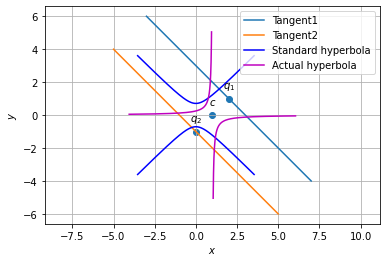
\includegraphics[width=\columnwidth]{./solutions/1/14/graph7.png}
	\caption{The standard and actual hyperbola.}
\end{figure}

\end{enumerate}

\item  $BE$ and $CF$ are two equal altitudes of a triangle $ABC$. Using RHS congruence rule, prove that the triangle $ABC$ is isosceles.
\item  $ABC$ is an isosceles triangle with $AB = AC$. Draw $AP \perp BC$ to show that $\angle  B = \angle  C$.
%
\item $\triangle ABC$ is an isosceles triangle in which $AB = AC$. Side $BA$ is produced to $D$ such that $AD = AB$. Show that $\angle BCD$ is a right angle.
%
\item $ABC$ is a right angled triangle in which $\angle A$ = 90$\degree$ and $AB = AC$. Find $\angle B$ and $\angle C$.
%
\item Show that in a right angled triangle, the hypotenuse is the longest side.
\item Sides AB and AC of $\triangle  ABC$ are extended to points P and Q respectively. Also, $\angle  PBC < \angle  QCB$. Show that $AC > AB$.

\item Line segments $AD$ and $BC$ intersect at $O$ and form $\triangle OAB$ and $\triangle ODC$. $\angle  B < \angle  A$ and $\angle  C < \angle  D$. Show that $AD < BC$.

\item $AB$ and $CD$ are respectively the smallest and longest sides of a quadrilateral $ABCD$. Show that $\angle  A > \angle  C$ and $\angle  B > \angle  D$.
%
\item In $\triangle PQR,  PR > PQ$ and $PS$ bisects $\angle  QPR$. Prove that $\angle  PSR > \angle  PSQ$.
%
\begin{enumerate}
\begin{figure}[!ht]
\centering
\resizebox{\columnwidth}{!}{\renewcommand{\theequation}{\theenumi}
\begin{enumerate}[label=\thesubsection.\arabic*.,ref=\thesubsection.\theenumi]
\numberwithin{equation}{enumi}
	%
%
\item 
%
Draw a circle of radius 3 units.Take two points P and Q on one its extended diameter each at a distance of 7 units from its centre. Draw tangents to the circle from these two points P and Q. 
\\
\solution The given parameters are listed in Table \ref{tab:table1}
%
\begin{table}[!ht]
\begin{center}
\begin{tabular}{ | m{2cm} | m{2cm} |} 
\hline
 & Circle \\
\hline
Centre  & $\vec{O}$=\myvec{0\\0} \\ 
\hline
Radius & $r$=3  \\ 
\hline
Radius & $d$=7  \\ 
\hline
\end{tabular}
\end{center}
\caption{Input values}
\label{tab:table1}
\end{table}
%
\begin{lemma}
  \label{lemma/linman/circ/contact/final}
  The points of contact for the tangent drawn from a point 
%
\begin{align}
  \vec{P} = d\vec{e}_1, \text{ where } \vec{e}_1 = \myvec{1\\0}
  \end{align}
  %
  to the circle are given by 
  \begin{align}
    \vec{x} = \frac{r^2}{d}\vec{e}_1  \pm r\sqrt{1 - \frac{r^2}{d^2}} \vec{e}_2
    \label{linman/circ/contact/final}
   \end{align}
%   
\end{lemma}
If $\vec{x}$ be a point of contact for the tangent from $\vec{P}$, 
\begin{align}
PR &\perp RO
\\
 \implies (\vec{O}-\vec{x})^{\top} (\vec{x}-\vec{P}) &= 0
 \\
 \text{or, }  \vec{P}^{\top} \vec{x} &=\norm{\vec{x}}^2 = r^2
 \\
 \implies \vec{e}_1^{\top} \vec{x} &= \frac{r^2}{d}
  \end{align}
  $\because \vec{O} = 0$.  The above equation can be expressed in parametric form as 
 \begin{align}
  \vec{x} = \frac{r^2}{d}\vec{e}_1 + \lambda \vec{e}_2
  \label{linman/circ/contact}
 \end{align}
 Substituting the above in 
 \begin{align}
  \norm{\vec{x}}^2 = r^2,
 \end{align}
 yields
\begin{align}
\norm{\frac{r^2}{d}\vec{e}_1 + \lambda \vec{e}_2}^2&=r^2
\\
\implies \lambda^2 &= r^2\sbrak{1 - \frac{r^2}{d^2}}
\\
\text{or, }\lambda &= \pm r\sqrt{1 - \frac{r^2}{d^2}}
\end{align}
%
Substituting $\lambda $ in \eqref{linman/circ/contact} yields \eqref{linman/circ/contact/final}.  Fig.  \ref{fig:Tangent lines to circle of radius 3 units.} shows all possible tangents
and their points of contact after substituting the numerical values in \eqref{linman/circ/contact/final}.
%
\begin{figure}[ht]
  \centering
  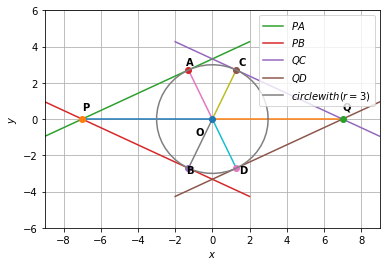
\includegraphics[width=\columnwidth]{solutions/su2021/circle/2/57/FIGURE3.png}
  \caption{Tangent lines to circle of radius 3 units.}
  \label{fig:Tangent lines to circle of radius 3 units.}
\end{figure}
%
\item Draw a  pair of tangents to a circle of radius 5 units  which are inclined to each other at an angle of $60\degree$.
\\
\solution  The angle between the tangents from $\vec{P}$ is given by 
\begin{lemma}
  Given a circle of radius $r$ and angle $\theta$ between the tangents, the intersection of the tangents and points of contact are
  given by Lemma   \ref{lemma/linman/circ/contact/final}  where 
  \begin{align}
    \implies d &= r\sin \frac{\theta}{2}
  \end{align}
%  
\end{lemma}
\begin{proof}
  From Fig.  \ref{fig:Tangent lines to circle of radius 3 units.},
\begin{align}
  \sin \frac{\theta}{2} &= \frac{r}{d}
  \\
  \implies d &= r\sin \frac{\theta}{2}
\end{align}
\end{proof}
Substituting numerical values and plotting, we obtain Fig. \ref{fig:Tangent lines to circle of radius 5 units.}.
%
\begin{figure}[ht]
  \centering
  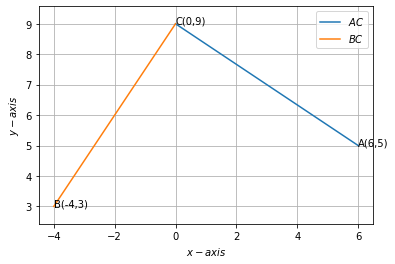
\includegraphics[width=\columnwidth]{solutions/su2021/circle/2/58/download.png}
  \caption{Tangent lines to circle of radius 5 units.}
  \label{fig:Tangent lines to circle of radius 5 units.}
\end{figure}   

\end{enumerate}
}
\caption{}
\label{fig:8.5.49_circle}	
\end{figure}
%
\item {\em Construction: }See Fig. \ref{fig:8.5.49_circle}.  The input parameters are
%
\begin{align}
\label{eq:8.5.49_constr_o}
\vec{O} &= \myvec{0\\0} 
\\
\vec{C} &= \myvec{r\\0} 
\label{eq:8.5.49_constr_c}
\end{align}
Then, 
%
\begin{align}
\label{eq:8.5.49_constr_a}
\vec{A} &= r\myvec{\cos \beta \\ -\sin \beta} 
\end{align}

\subitem Equal chords subtend equal angles at the centre.  Hence 
\begin{align}
\phase{EOC} &= \phase{AOD} = \frac{360 \degree - \alpha -\beta}{2}
\\
&= 180\degree - \frac{\alpha+\beta}{2}
\end{align}
Thus, 
\begin{align}
\vec{D} &= r\myvec{\cos \brak{180^{\circ}-\frac{\alpha+\beta}{2}+\alpha} \\ \sin \brak{180^{\circ}-\frac{\alpha+\beta}{2}+\alpha}} 
\\
 &= r\myvec{-\cos \frac{\alpha-\beta}{2} \\ -\sin \frac{\alpha-\beta}{2}}
\label{eq:8.5.49_constr_d}
\\
\vec{E} &= r\myvec{\cos \brak{180^{\circ}-\frac{\alpha+\beta}{2}} \\ \sin \brak{180^{\circ}-\frac{\alpha+\beta}{2}}}
\\
 &= r\myvec{-\cos \frac{\alpha+\beta}{2} \\ \sin \frac{\alpha+\beta}{2}}
\label{eq:8.5.49_constr_e}
\end{align}
\subitem $\vec{B}$ can be found as the intersection of $AD$ and $CE$.

The given curve 
\begin{align}
	y =\frac{1}{x-1}
\end{align}
can be expressed as 
\begin{align}
	xy - y - 1 = 0 \label{eq:solutions/1/14/eq:hyperbola}
\end{align}
Hence, we have
\begin{align}
	\vec{V} = \frac{1}{2}\myvec{0 & 1 \\ 1 & 0}, 
	\vec{u} = \frac{1}{2}\myvec{0 \\-1},
	f = -1
\end{align}
Since $\mydet{\vec{V}} < 0$, the equation \eqref{eq:solutions/1/14/eq:hyperbola} represents hyperbola.
To find the values of $\lambda_1$ and $\lambda_2$, consider the characteristic equation,
\begin{align}
	\mydet{\lambda\vec{I} - \vec{V}} &= 0\\
	\implies \mydet{\myvec{\lambda & 0\\0 & \lambda} - \myvec{0 & \frac{1}{2} \\ \frac{1}{2} & 0}} &= 0\\
	\implies \mydet{ \lambda & \frac{-1}{2} \\ \frac{-1}{2} & \lambda} &= 0\\
	\implies \lambda_1 &= \frac{1}{2} , \lambda_2 = \frac{-1}{2}
\end{align}
In addition, given the slope -1, the direction and normal vectors are given by 
\begin{align}
	\vec{m} = \myvec{1 \\ -1} \\
	\vec{n} = \myvec{ 1 \\ 1}
\end{align}
The parameters of hyperbola are as follows:
\begin{align}
	\vec{c} &= -\vec{V}^{-1}\vec{u} \\
	&= -\myvec{0 & 2\\ 2 & 0}\myvec{0 \\ -\frac{1}{2}} \\
	&= \myvec{1 \\ 0}\\
	axes &= \begin{cases}
	\sqrt{\frac{\vec{u}^T\vec{V}^{-1}\vec{u} - f}{\lambda_1}} = \sqrt{2}\\
 \sqrt{\frac{f-\vec{u}^T\vec{V}^{-1}\vec{u}}{\lambda_2}} = \sqrt{2}
\end{cases}
\end{align}
which represents the standard hyperbola equation,
\begin{align}
	\frac{x^2}{2} - \frac{x^2}{2} = 1
\end{align}
The points of contact are given by 
\begin{align}
  \tiny{K} &=\pm \sqrt{\frac{\vec{u}^T\vec{V}^{-1}\vec{u} - f}{\vec{n}^T\vec{V}^{-1}\vec{n}}}
  = \pm \frac{1}{2}\\
  \vec{q} &= \vec{V}^{-1}(k\vec{n}-\vec{u})\\
  \vec{q_1} &= \myvec{0 & 2\\2 & 0} \sbrak{\frac{1}{2}\myvec{1 \\ 1} - \myvec{0\\ \frac{-1}{2}}}\\
  &= \myvec{2 \\ 1}\\
  \vec{q_2} &= \myvec{0 & 2\\2 & 0} \sbrak{\frac{-1}{2}\myvec{1 \\ 1} - \myvec{0\\ \frac{-1}{2}}}\\
  &= \myvec{0 \\ -1}
\end{align} 
$\therefore$ The tangents are given by
\begin{align}
	\myvec{1 & 1} \brak{\vec{x} - \myvec{2 \\ 1}} = 0 \\
	\myvec{1 & 1} \brak{\vec{x} - \myvec{0 \\ -1}} = 0
\end{align}
The desired equations of all lines having slope -1 that are tangents to the curve $\frac{1}{x-1}, x \neq 1$ are given by
\begin{align}
	\myvec{1 & 1}\vec{x} &= 3 \\
	\myvec{1 & 1}\vec{x} &= -1 
\end{align}
The above results are verified in the following figure.
\begin{figure}[h!] \label{eq:solutions/1/14/fig:tangents}
	\centering
	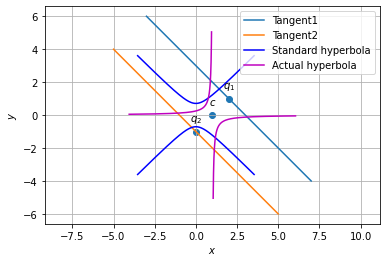
\includegraphics[width=\columnwidth]{./solutions/1/14/graph7.png}
	\caption{The standard and actual hyperbola.}
\end{figure}

\end{enumerate}

\item Show that of all line segments drawn from a given point not on it, the perpendicular line segment is the shortest.
%
\item $ABCD$ is a trapezium with $AB  \parallel  DC$. $E$ and $F$ are points on non-parallel sides $AD$ and $BC$ respectively such that $EF$ is parallel to $AB$
. Show that
$\frac{AE}{ED}=\frac{ BF}{  FC}$ .
\begin{enumerate}
\begin{figure}[!ht]
\centering
\resizebox{\columnwidth}{!}{%Exercise 8.1 prob 47
\begin{tikzpicture}
[scale=0.5,>=stealth,point/.style={draw,circle,fill = black,inner sep=0.5pt},]
%\tikzset{shift={(-3,0)}}
%Triangle sides
\def\a{4}
\def\c{9}
\def\xA{4}
\def\h{3}
\def\k{1}
%\def\c{7.5}
\def\yE{\h/2}
%Labeling points
\node (D) at (0,0)[point,label=below left:$D$] {};
\node (B) at ({\xA+\a}, \h )[point,label=above right:$B$] {};
\node (C) at (\c, 0)[point,label=below right:$C$] {};
%\node (E) at (2, \yE)
%\node (F) at (8.5, \yE)[point,label=below right:$F$] {};
%\node (M) at (\xA,\yE)[point,label=above right:$M$] {};
%\node (N) at ({\xA+\a}, \yE)[point,label=above left:$N$] {};
%\node (X) at (\xA , 0)[point,label=below left:$X$] {};
%\node (Y) at ({\xA+\a}, 0)[point,label=below right:$Y$] {};
\node (A) at (\xA , \h)[point,label=above left:$A$] {};
\node (E) at ($(D)!0.5!(A)$)[point,label=above left:$E$] {};
\node (F) at ($(B)!0.5!(C)$)[point,label=above right:$F$] {};



%A



%Drawing parallelogram ABCD
\draw (A) -- (B)--(C) --(D)--(A);
%\draw (A) --(X);
\draw (E) --(F);
\draw(A)--node[right]{$\textrm{k}$} (E)--node[right]{$\textrm{1}$} (D);
\draw(B)--node[left]{$\textrm{m}$} (F)--node[left]{$\textrm{1}$} (C);


%\draw (B) --(Y);
%marking right angles
%\tkzMarkRightAngle[fill=green!20,size=.2](D,X,A)
%\tkzMarkRightAngle[fill=green!20,size=.2](C,Y,B)


%
\end{tikzpicture}
}
\caption{}
\label{fig:8.1.47_trapezium_ABCD}	
\end{figure}

\item {\em Construction: }See Fig. \ref{fig:8.1.47_trapezium_ABCD}.
The input parameters are
\begin{align}
\label{eq:8.1.47_constr_d}
\vec{D} &= \myvec{0\\0} 
\\
\vec{C} &= \myvec{c\\0} 
\\
\vec{A} &= \myvec{p\\q} 
\\
\vec{B} &= \myvec{b\\q}, \quad b < c 
\label{eq:8.1.47_constr_c}
\end{align}
%
For $0 < k < 1$, 
\begin{align}
\label{eq:8.1.47_constr_e}
\vec{E} &= \frac{{k\vec{D} +\vec{A}}}{k+1}
\\
\vec{F} &= \frac{{k\vec{C} +\vec{B}}}{k+1}
\label{eq:8.1.47_constr_f}
\end{align}


The given curve 
\begin{align}
	y =\frac{1}{x-1}
\end{align}
can be expressed as 
\begin{align}
	xy - y - 1 = 0 \label{eq:solutions/1/14/eq:hyperbola}
\end{align}
Hence, we have
\begin{align}
	\vec{V} = \frac{1}{2}\myvec{0 & 1 \\ 1 & 0}, 
	\vec{u} = \frac{1}{2}\myvec{0 \\-1},
	f = -1
\end{align}
Since $\mydet{\vec{V}} < 0$, the equation \eqref{eq:solutions/1/14/eq:hyperbola} represents hyperbola.
To find the values of $\lambda_1$ and $\lambda_2$, consider the characteristic equation,
\begin{align}
	\mydet{\lambda\vec{I} - \vec{V}} &= 0\\
	\implies \mydet{\myvec{\lambda & 0\\0 & \lambda} - \myvec{0 & \frac{1}{2} \\ \frac{1}{2} & 0}} &= 0\\
	\implies \mydet{ \lambda & \frac{-1}{2} \\ \frac{-1}{2} & \lambda} &= 0\\
	\implies \lambda_1 &= \frac{1}{2} , \lambda_2 = \frac{-1}{2}
\end{align}
In addition, given the slope -1, the direction and normal vectors are given by 
\begin{align}
	\vec{m} = \myvec{1 \\ -1} \\
	\vec{n} = \myvec{ 1 \\ 1}
\end{align}
The parameters of hyperbola are as follows:
\begin{align}
	\vec{c} &= -\vec{V}^{-1}\vec{u} \\
	&= -\myvec{0 & 2\\ 2 & 0}\myvec{0 \\ -\frac{1}{2}} \\
	&= \myvec{1 \\ 0}\\
	axes &= \begin{cases}
	\sqrt{\frac{\vec{u}^T\vec{V}^{-1}\vec{u} - f}{\lambda_1}} = \sqrt{2}\\
 \sqrt{\frac{f-\vec{u}^T\vec{V}^{-1}\vec{u}}{\lambda_2}} = \sqrt{2}
\end{cases}
\end{align}
which represents the standard hyperbola equation,
\begin{align}
	\frac{x^2}{2} - \frac{x^2}{2} = 1
\end{align}
The points of contact are given by 
\begin{align}
  \tiny{K} &=\pm \sqrt{\frac{\vec{u}^T\vec{V}^{-1}\vec{u} - f}{\vec{n}^T\vec{V}^{-1}\vec{n}}}
  = \pm \frac{1}{2}\\
  \vec{q} &= \vec{V}^{-1}(k\vec{n}-\vec{u})\\
  \vec{q_1} &= \myvec{0 & 2\\2 & 0} \sbrak{\frac{1}{2}\myvec{1 \\ 1} - \myvec{0\\ \frac{-1}{2}}}\\
  &= \myvec{2 \\ 1}\\
  \vec{q_2} &= \myvec{0 & 2\\2 & 0} \sbrak{\frac{-1}{2}\myvec{1 \\ 1} - \myvec{0\\ \frac{-1}{2}}}\\
  &= \myvec{0 \\ -1}
\end{align} 
$\therefore$ The tangents are given by
\begin{align}
	\myvec{1 & 1} \brak{\vec{x} - \myvec{2 \\ 1}} = 0 \\
	\myvec{1 & 1} \brak{\vec{x} - \myvec{0 \\ -1}} = 0
\end{align}
The desired equations of all lines having slope -1 that are tangents to the curve $\frac{1}{x-1}, x \neq 1$ are given by
\begin{align}
	\myvec{1 & 1}\vec{x} &= 3 \\
	\myvec{1 & 1}\vec{x} &= -1 
\end{align}
The above results are verified in the following figure.
\begin{figure}[h!] \label{eq:solutions/1/14/fig:tangents}
	\centering
	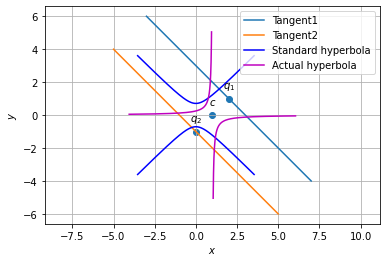
\includegraphics[width=\columnwidth]{./solutions/1/14/graph7.png}
	\caption{The standard and actual hyperbola.}
\end{figure}

\end{enumerate}

\item $ST$ is a line joining two points on $PQ$ and $PR$ in $\triangle PQR$.  If $\frac{PS}{ SQ}=\frac{PT}{ TR}$ and $ \angle  PST = \angle  PRQ$, prove that $PQR$ is an isosceles triangle.
%
\item If $LM  \parallel  CB$ and $LN  \parallel  CD$, prove that $\frac{AM}{AB} = \frac{ AN}{AD}$.
%
\item $D$ is a point on $AB$ and $E, F$ are points on $BC$ such that $DE  \parallel  AC$ and $DF  \parallel  AE$. Prove that $\frac{BF} {FE} =\frac{BE}  {EC}$.
%
\item $O$ is a point in the interior of $\triangle ABC$. $D$ is a point on $OA$.  If $DE  \parallel  OB$ and $DF  \parallel  OC$. Show that $EF  \parallel  BC$.
\begin{enumerate}
\begin{figure}[!ht]
\centering
\resizebox{\columnwidth}{!}{%Exercise 8.1 prob 47
\begin{tikzpicture}
[scale=0.5,>=stealth,point/.style={draw,circle,fill = black,inner sep=0.5pt},]
%\tikzset{shift={(-3,0)}}
%Triangle sides
\def\a{4}
\def\c{9}
\def\xA{4}
\def\h{3}
\def\k{1}
%\def\c{7.5}
\def\yE{\h/2}
%Labeling points
\node (D) at (0,0)[point,label=below left:$D$] {};
\node (B) at ({\xA+\a}, \h )[point,label=above right:$B$] {};
\node (C) at (\c, 0)[point,label=below right:$C$] {};
%\node (E) at (2, \yE)
%\node (F) at (8.5, \yE)[point,label=below right:$F$] {};
%\node (M) at (\xA,\yE)[point,label=above right:$M$] {};
%\node (N) at ({\xA+\a}, \yE)[point,label=above left:$N$] {};
%\node (X) at (\xA , 0)[point,label=below left:$X$] {};
%\node (Y) at ({\xA+\a}, 0)[point,label=below right:$Y$] {};
\node (A) at (\xA , \h)[point,label=above left:$A$] {};
\node (E) at ($(D)!0.5!(A)$)[point,label=above left:$E$] {};
\node (F) at ($(B)!0.5!(C)$)[point,label=above right:$F$] {};



%A



%Drawing parallelogram ABCD
\draw (A) -- (B)--(C) --(D)--(A);
%\draw (A) --(X);
\draw (E) --(F);
\draw(A)--node[right]{$\textrm{k}$} (E)--node[right]{$\textrm{1}$} (D);
\draw(B)--node[left]{$\textrm{m}$} (F)--node[left]{$\textrm{1}$} (C);


%\draw (B) --(Y);
%marking right angles
%\tkzMarkRightAngle[fill=green!20,size=.2](D,X,A)
%\tkzMarkRightAngle[fill=green!20,size=.2](C,Y,B)


%
\end{tikzpicture}
}
\caption{}
\label{fig:8.1.47_trapezium_ABCD}	
\end{figure}

\item {\em Construction: }See Fig. \ref{fig:8.1.47_trapezium_ABCD}.
The input parameters are
\begin{align}
\label{eq:8.1.47_constr_d}
\vec{D} &= \myvec{0\\0} 
\\
\vec{C} &= \myvec{c\\0} 
\\
\vec{A} &= \myvec{p\\q} 
\\
\vec{B} &= \myvec{b\\q}, \quad b < c 
\label{eq:8.1.47_constr_c}
\end{align}
%
For $0 < k < 1$, 
\begin{align}
\label{eq:8.1.47_constr_e}
\vec{E} &= \frac{{k\vec{D} +\vec{A}}}{k+1}
\\
\vec{F} &= \frac{{k\vec{C} +\vec{B}}}{k+1}
\label{eq:8.1.47_constr_f}
\end{align}


The given curve 
\begin{align}
	y =\frac{1}{x-1}
\end{align}
can be expressed as 
\begin{align}
	xy - y - 1 = 0 \label{eq:solutions/1/14/eq:hyperbola}
\end{align}
Hence, we have
\begin{align}
	\vec{V} = \frac{1}{2}\myvec{0 & 1 \\ 1 & 0}, 
	\vec{u} = \frac{1}{2}\myvec{0 \\-1},
	f = -1
\end{align}
Since $\mydet{\vec{V}} < 0$, the equation \eqref{eq:solutions/1/14/eq:hyperbola} represents hyperbola.
To find the values of $\lambda_1$ and $\lambda_2$, consider the characteristic equation,
\begin{align}
	\mydet{\lambda\vec{I} - \vec{V}} &= 0\\
	\implies \mydet{\myvec{\lambda & 0\\0 & \lambda} - \myvec{0 & \frac{1}{2} \\ \frac{1}{2} & 0}} &= 0\\
	\implies \mydet{ \lambda & \frac{-1}{2} \\ \frac{-1}{2} & \lambda} &= 0\\
	\implies \lambda_1 &= \frac{1}{2} , \lambda_2 = \frac{-1}{2}
\end{align}
In addition, given the slope -1, the direction and normal vectors are given by 
\begin{align}
	\vec{m} = \myvec{1 \\ -1} \\
	\vec{n} = \myvec{ 1 \\ 1}
\end{align}
The parameters of hyperbola are as follows:
\begin{align}
	\vec{c} &= -\vec{V}^{-1}\vec{u} \\
	&= -\myvec{0 & 2\\ 2 & 0}\myvec{0 \\ -\frac{1}{2}} \\
	&= \myvec{1 \\ 0}\\
	axes &= \begin{cases}
	\sqrt{\frac{\vec{u}^T\vec{V}^{-1}\vec{u} - f}{\lambda_1}} = \sqrt{2}\\
 \sqrt{\frac{f-\vec{u}^T\vec{V}^{-1}\vec{u}}{\lambda_2}} = \sqrt{2}
\end{cases}
\end{align}
which represents the standard hyperbola equation,
\begin{align}
	\frac{x^2}{2} - \frac{x^2}{2} = 1
\end{align}
The points of contact are given by 
\begin{align}
  \tiny{K} &=\pm \sqrt{\frac{\vec{u}^T\vec{V}^{-1}\vec{u} - f}{\vec{n}^T\vec{V}^{-1}\vec{n}}}
  = \pm \frac{1}{2}\\
  \vec{q} &= \vec{V}^{-1}(k\vec{n}-\vec{u})\\
  \vec{q_1} &= \myvec{0 & 2\\2 & 0} \sbrak{\frac{1}{2}\myvec{1 \\ 1} - \myvec{0\\ \frac{-1}{2}}}\\
  &= \myvec{2 \\ 1}\\
  \vec{q_2} &= \myvec{0 & 2\\2 & 0} \sbrak{\frac{-1}{2}\myvec{1 \\ 1} - \myvec{0\\ \frac{-1}{2}}}\\
  &= \myvec{0 \\ -1}
\end{align} 
$\therefore$ The tangents are given by
\begin{align}
	\myvec{1 & 1} \brak{\vec{x} - \myvec{2 \\ 1}} = 0 \\
	\myvec{1 & 1} \brak{\vec{x} - \myvec{0 \\ -1}} = 0
\end{align}
The desired equations of all lines having slope -1 that are tangents to the curve $\frac{1}{x-1}, x \neq 1$ are given by
\begin{align}
	\myvec{1 & 1}\vec{x} &= 3 \\
	\myvec{1 & 1}\vec{x} &= -1 
\end{align}
The above results are verified in the following figure.
\begin{figure}[h!] \label{eq:solutions/1/14/fig:tangents}
	\centering
	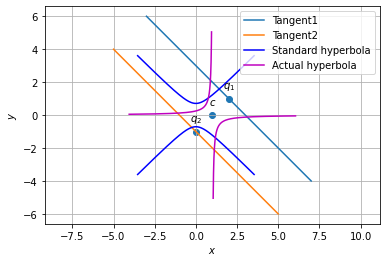
\includegraphics[width=\columnwidth]{./solutions/1/14/graph7.png}
	\caption{The standard and actual hyperbola.}
\end{figure}

\end{enumerate}

\item $O$ is a point in the interior of $\triangle PQR$.  $A, B and C$ are points on $OP, OQ$ and $OR$ respectively such that $AB  \parallel  PQ$ and $AC  \parallel  PR$. Show that $BC  \parallel  QR$.
%
\item $ABCD$ is a trapezium in which $AB  \parallel  DC$ and its diagonals intersect each other at the point $O$. Show
that
$\frac{AO}{ BO}=\frac{CO}{  DO}$
%
\item The diagonals of a quadrilateral $ABCD$ intersect each other at the point $O$ such that $\frac{AO}{ BO}=\frac{CO}{  DO}$.   Show that $ABCD$ is a trapezium.
%
\item $PQ \parallel RS$ and $PS$ intersects $QR$ at $O$.  Show that $\triangle OPQ \sim \triangle ORS$.
 \item $CM$ and $RN$ are respectively the medians of $ \triangle  ABC$ and $ \triangle  PQR$. If $ \triangle  ABC  \sim   \triangle  PQR$, prove that 
\begin{enumerate}
\item  $ \triangle  AMC  \sim   \triangle  PNR$ 
\item  $\frac{CM}{RN}=\frac{ AB}{  PQ}$
\item $ \triangle  CMB  \sim   \triangle  RNQ$
%
\end{enumerate}
\item Diagonals $AC$ and $BD$ of a trapezium $ABCD$ with $AB  \parallel  DC$ intersect each other at the point $O$. Using a similarity criterion for two triangles, show that
$\frac{OA}{OC} =  \frac{OB}  {OD}$
%
\item In $\triangle PQR$, $QP$ is extended to $T$ and $S$ is a point on $QR$ such that $ \frac{QR}{QS}=\frac{ QT}{  PR}$. If $\angle PRQ = \angle PQS$, show that 
 that  $\triangle  PQS  \sim   \triangle  TQR$.
\item $S$ and $T$ are points on sides $PR$ and $QR$ of $\triangle PQR$ such that $\angle P = \angle 
 RTS$. Show that $\triangle RPQ \sim \triangle RTS$.
\item  In $\triangle ABC$, $D$ and $E$ are points on the sides $AB$ and $AC$ respectively.  If  $\triangle  ABE \cong   \triangle  ACD$, show that  $\triangle  ADE  \sim   \triangle  ABC$.
\item   Altitudes $AD$ and CE of  $\triangle  ABC$ intersect each other at the point $P$. Show that:
%
\begin{enumerate}
\item   $\triangle  AEP  \sim   \triangle  CDP $
\item   $\triangle  ABD  \sim   \triangle  CBE $
\item   $\triangle  AEP  \sim   \triangle  ADB$
 \item  $\triangle  PDC  \sim   \triangle  BEC$
\end{enumerate}
%
\item  $E$ is a point on the side $AD$ produced of a parallelogram $ABCD$ and $BE$ intersects $CD$ at $F$. Show that  $\triangle  ABE  \sim   \triangle  CFB$.
\item  $ABC$ and $AMP$ are two right triangles, right angled at $B$ and $M$ respectively. $M$ lies on $AC$ and $AB$ is extended to meet $P$. Prove that: 
\begin{enumerate}
\item   $\triangle  ABC  \sim   \triangle  AMP$
\item  $\frac{CA}{PA} = \frac{BC}{  MP}$
\end{enumerate}
%
\item  $CD$ and $GH$ are respectively the bisectors of  $\angle  ACB$ and  $\angle  EGF$ such that $D$ and $H$ lie on sides $AB$ and $FE$ of  $\triangle  ABC$ and  $\triangle  EFG$ respectively. If  $\triangle  ABC  \sim   \triangle  FEG$, show that:
\item  $\frac{CD}{GH} = \frac{ AC}{  FG}$
\item  $ \triangle  DCB  \sim   \triangle  HGE$
 \item  $ \triangle  DCA  \sim   \triangle  HGF$
\item  $E$ is a point on side $CB$ produced of an isosceles $\triangle ABC$ with $AB = AC$. If $AD  \perp  BC$ and $EF  \perp  AC$, prove that  $\triangle  ABD  \sim   \triangle  ECF$.
\item  Sides $AB$ and $BC$ and median $AD$ of a $\triangle ABC$ are respectively proportional to sides  $PQ$  and $QR$ and median $PM$ of  $\triangle PQR$. Show that  $\triangle  ABC  \sim  \triangle PQR$ .
\item  $D$ is a point on the side $BC$ of a $\triangle ABC$ such that  $\angle  ADC =  \angle  BAC$. Show that $CA^2 = CB.CD$.
\item  Sides $AB$ and $AC$ and median $AD$ of a $\triangle ABC$ are respectively proportional to sides $PQ$ and $PR$ and median $PM$ of another $\triangle PQR$. Show that  $\triangle  ABC  \sim   \triangle PQR$ .%
\item  If $AD$ and $PM$ are medians of $\triangle s ABC$ and $PQR$, respectively where  $\triangle  ABC  \sim   \triangle PQR$ , prove that
$\frac{AB}{ PQ} = \frac{AD}{  PM}$
\item The line segment $XY$ is parallel to side $AC$ of  $\triangle  ABC$ and it divides the triangle into two parts of equal areas. Find the ratio
$\frac{AX}{ AB}$
% 
\item  Diagonals of a trapezium $ABCD$ with $AB  \parallel  DC$ intersect each other at the point $O$. If $AB = 2 CD$, find the ratio of the areas of $\triangle s AOB$ and $COD$.
\item  $ABC$ and $DBC$ are two triangles on the same base $BC$. If $AD$ intersects $BC$ at $O$, show that
$\frac{ar (ABC)}{ ar (DBC)}=\frac{AO}{  DO}$.
\item  If the areas of two similar triangles are equal, prove that they are congruent.
\item  $D, E$ and $F$ are respectively the mid-points of sides $AB$, $BC$ and $CA$ of  $\triangle  ABC$. Find the ratio of the areas of  $\triangle  DEF$ and  $\triangle  ABC$.
\item  Prove that the ratio of the areas of two similar triangles is equal to the square of the ratio of their corresponding medians.
\item  Prove that the area of an equilateral triangle described on one side of a square is equal to half the area of the equilateral triangle described on one of its diagonals.
\item $ABC$ and $BDE$ are two equilateral triangles such that $D$ is the mid-point of $BC$. Find the ratio of the areas of triangles $ABC$ and $BDE$.
\item The sides of two similar triangles are in the ratio 4 : 9. Find the ratio the area of  these triangles are in the ratio
\item In $\triangle ABC, \angle  ACB = 90\degree$ and $CD  \perp  AB$. Prove that 
$\frac{BC^2}{AC^2} = \frac{BD}{ AD}$.
\item In $\triangle ABC$,  if $AD  \perp  BC$, prove that $AB^2+ CD^2 = BD^2 + AC^2$.
\item $BL$ and $CM$ are medians of a $\triangle ABC$ right angled at $A$. Prove that $4 (BL^2 + CM^2
) = 5 BC^2$ .
\item $O$ is any point inside a rectangle $ABCD$. Prove that $OB^2+OD^2 = OA^2+OC^2$.
\item  $PQR$ is a triangle right angled at $P$ and $M$ is a point on $QR$ such that $PM  \perp  QR$. Show that $PM^2= QM . MR$.
\item  $ABD$ is a triangle right angled at $A$ and $AC \perp  BD$. Show that
\begin{enumerate}
\item  $AB^2 = BC . BD$
\item  $AC^2 = BC . DC$
\item  $AD^2  = BD . CD$
\end{enumerate}
\item  $ABC$ is an isosceles triangle right angled at $C$. Prove that $AB^2= 2 AC^2$.
 \item  $ABC$ is an isosceles triangle with $AC = BC$. If $AB^2=2 AC^2$, prove that $ABC$ is a right triangle.
\item  $ABC$ is an equilateral triangle of side $2a$. Find each of its altitudes. 
\item  Prove that the sum of the squares of the sides of a rhombus is equal to the sum of the squares of its diagonals.
\item  $O$ is a point in the interior of a $\triangle ABC, OD  \perp  BC, OE  \perp  AC and OF  \perp  AB$. Show that
%
\begin{enumerate}
\item  $OA^2 + OB^2 + BD^2 – OD2 – OE2– OF2 = AF^2 + BD^2 + CE^2$.
\item  $AF^2 + BD^2 +CE^2 = AE^2 + CD^2 + BF^2$.
\end{enumerate}
\item  $D$ and $E$ are points on the sides $CA$ and $CB$ respectively of a $\triangle ABC$ right angled at $C$. Prove that $AE^2+ BD^2 = AB^2 + DE^2$.
\item  The perpendicular from $A$ on side $BC$ of a  $\triangle  ABC$ intersects $BC$ at $D$ such that $DB = 3 CD$. Prove that $2 AB^2= 2 AC^2 + BC^2$ .
\item  In an equilateral $\triangle ABC$, $D$ is a point on side $BC$ such that $BD = \frac{1}{3} BC$.  Prove that $9 AD^2= 7 AB^2$.
\item  In an equilateral triangle, prove that three times the square of one side is equal to four times the square of one of its altitudes.
\item  $PS$ is the bisector of  $\angle  QPR$ of  $\triangle PQR$ . Prove that
$\frac{QS}{SR} = \frac{PQ}{PR}$
\item $D$ is a point on hypotenuse $AC$ of  $\triangle  ABC$, such that $BD  \perp  AC, DM  \perp  BC$ and $DN  \perp  AB$. Prove that :
\begin{enumerate}
\item  DM2 = DN . MC  
 \item  DN2 = DM . AN
\end{enumerate}

\item  $ABC$ is a triangle in which  $\angle  ABC > 90\degree$ and $AD  \perp  CB$ produced. Prove that
$ AC^2= AB^2 + BC^2 + 2 BC . BD$.
\item $ABC$ is a triangle in which  $\angle  ABC < 90\degree$ and $AD  \perp  BC$. Prove that $AC^2= AB^2 + BC^2 – 2 BC . BD$.
\item $AD$ is a median of a $\triangle ABC$ and $AM  \perp  BC$. Prove that :
\begin{enumerate}
\item  $AC^2 = AD^2 + BC . DM +
\brak{\frac{BC}{ 2}}^2$
\item  $AB^2 = AD^2 – BC . DM + \brak{\frac{BC}{ 2}}^
2 $
\item  $AC^2 + AB^2 = 2 AD^2 + \frac{1}{ 2} BC^2$
\end{enumerate}
\item Prove that the sum of the squares of the diagonals of parallelogram is equal to the sum of the squares of its sides.
\item   $D$ is a point on side $BC$ of  $\triangle  ABC$ such that
$\frac{BD}{CD} \frac{AB}{AC}  $.  Prove that $AD$ is the bisector of  $\angle  BAC$.
\end{enumerate}


